\label{chap:metodologia}
Neste capítulo descrevemos o MetaStream, um \textit{framework} para seleção periódica de algoritmos. Também apresentaremos os meta-atributos utilizados, justificativas, configurações do \textit{framework}, incluindo os algoritmos a nível base analisador, o meta-classificador, LightGBM em configurações incremental e não-incremental e as respectivas avaliações nos experimentos.

\begin{figure}[ht]
    \centering
    \includegraphics[width=0.7\linewidth]{general_diag}
    \caption{Diagrama de operação do MetaStream.}
    \label{fig:general_diag}
\end{figure}

\section{Metastream}
\label{sec:metastream}

Em ambientes de fluxos de dados, o espaço de instância de problemas é composto
por apenas um problema $p$ enquanto os meta-atributos $F$ são extraídos dos
dados de cada janela temporal para compor o meta-exemplo.
É importante que o processo de extração dos meta-atributos tenha baixo custo
computacional e alto grau de informação.
Além disso, a  performance desses algoritmos $A$ são obtidas de forma periódica para cada janela deslizante. Portanto, o algoritmo atual é substituído logo que o meta-modelo prediz que um
algoritmo diferente é mais adequado para os exemplos da próxima janela
deslizante. Essa é uma abordagem padrão na literatura de MtA em fluxos de dados
\cite{read2012batch, vanrijn2014algorithm, Anderson2019}.

A literatura apresenta alternativas a seleção de algoritmos (ou modelos)
baseado em MtA para mudança de conceito. Um dos primeiros a apresentar é R.
Klinkenberg (2005) \cite{klinkenberg2005}, em que características obtidas do
processo de aprendizado em si, no caso o tamanho das janelas deslizantes, foram
usadas para induzir meta-modelos.
Uma abordagem diferente foi investigada por J. Gama and P. Kosina (2014)
\cite{gama2014} e R. Anderson et al. (2019) \cite{Anderson2019}
reusando modelos previamente aprendidos mas usando o mesmo algoritmo para
induzir esses modelos no fluxo de dados. Uma terceira alternativa é dada por J.
N. van Rijn et al. (2018) \cite{VanRijn2018}, em que conjuntos de
modelos são usados, tendo um alto custo computacional para induzir modelos para cada
algoritmo e para manter os pesos atualizados.

Em seguida, é apresentado o MetaStream baseado no trabalho de A. L. D. Rossi et
al. (2014) \cite{rossi2014metastream}, que têm fases \textit{offline} e \textit{online}.
A fase \textit{offline} é projetada para escolha de hiper-parâmetros, validação e
treinamento e geração dos dados em lote. A fase \textit{online} age no ambiente dinâmico, recomendando um algoritmo para uma dada janela de dados. Ambas as fases são baseadas em sistemas de recomendação de MtA.


\subsection{Fase \textit{offline}}
\label{subsec:offline}
Essa fase se inicia aguardando o fluxo de dados gerar um lote de tamanho
razoável para indução e seleção de modelos base, com esse lote em mãos, é
realizada uma validação cruzada \textit{k-fold} para estimar os
hiper-parâmetros dos algoritmos base, aqui assumindo que tais hiper-parâmetros
serão os melhores para os eventos futuros.
Após isso, em um configuração de janelas deslizantes, como mostrado na Figura
\ref{fig:ms_diag0_off}, uma janela $\omega_{b1}$ é usada para induzir modelos
com os algoritmos de nível base e também os meta-atributos $x^m$ também são
extraídos dessa janela.

\begin{figure}[ht]
    \centering
    \includegraphics[width=0.7\linewidth]{ms_diag0_off}
    \caption{Extração de meta-atributos da janela $\omega_b$ e obtenção de
    rótulo da janela $\eta_b$.}
    \label{fig:ms_diag0_off}
\end{figure}

Em seguida, os modelos induzidos são avaliados nos exemplos da janela
$\eta_{b1}$, em que o algoritmo que produziu o modelo de melhor performance
preditiva é definido como rótulo de $y^m$. Esse processo gera o primeiro
meta-exemplo. O mesmo processo é aplicado continuamente por $N$ passos, onde
$N$ é o número mínimo de instâncias para induzir um modelo consistente para
gerar os meta-dados iniciais. Esses $N$ meta-exemplos serão os primeiros dados
que serão usados para induzir modelos na fase \textit{online}.

\subsection{Fase \textit{online}}
\label{subsec:online}

A fase \textit{online} é iniciada quando o \textit{framework} começa a receber um contínuo fluxo de dados.
Inicialmente, ele recebe um vetor de atributos $\boldsymbol{x}_b =
(x_1,...,x_p)$, e após algum atraso, o rótulo $y_b \in \{0,1,..,k\}$
dessa instância, onde $k$ é o número de classes para uma tarefa de classificação ou $y_b \in \rm{I\!R}$ para
regressão.

A Figura \ref{fig:ms_diagram0} mostra um dado momento $t$ na fase \textit{online}. Ele
tem uma janela de tamanho fixo $\omega_b$ que será usado para induzir um
modelo, uma janela de tamanho fixo $\eta_b$ em que o modelo induzido em
$\omega_b$ será avaliado assim que o rótulo referente for descoberto, um
tamanho $\gamma_b$ que é o atraso em observar o rótulo para os exemplos na
janela $\eta_b$ e uma janela de tamanho variável $\lambda_b$ de exemplos
aguardando serem processados.
Quando $\gamma_b$ tem o mesmo tamanho que $\eta_b$, isto é, todos os rótulos de
$\eta_b$ foram obtidos, a janela $\omega_b$ é deslizada $\eta_b$ instâncias
para a direita e um novo modelo é induzido nessa janela.

\begin{figure}[ht]
    \centering
    
\includegraphics[width=0.7\linewidth]{metastream_diag0}
    \caption{Discretização de janelas no nível base do fluxo de dados.}
    \label{fig:ms_diagram0}
\end{figure}

MtA entra em ação no segundo nível de processamento, nomeado nível meta. Como
mostrado na Figura \ref{fig:ms_diagram1}, os meta-atributos são extraídos da
janela $\omega_b$ e geram o meta-exemplo sem o rótulo que é mantido para
atualização posterior.

\begin{figure}[ht]
    \centering
    \includegraphics[width=0.7\linewidth]{metastream_diag1}
    \caption{Extração de meta-atributos das janelas  $\omega_b$ e $\eta_b$ no nível meta.}
    \label{fig:ms_diagram1}
\end{figure}

O algoritmo de aprendizado (meta-aprendiz) usa meta-exemplos rotulados
previamente na meta-base para induzir um meta-classificador, que é utilizado
para recomendar um algoritmo que induzirá um modelo usando a janela $\omega_b$
que provavelmente será o mais preciso para prever os rótulos dos exemplos em
$\eta_b$.

\section{Parâmetros}
\label{sec:params}

Como descrito na Seção \ref{sec:metalearning}, nosso problema de seleção de algoritmos é dada pela escolha do espaço de hipóteses mais apropriado para a janela de dados mais recente. Portanto, sob a presença de mudança de conceito, é esperado que a metodologia aqui descrita consiga recomendar um classificador alternativo que se ajuste melhor aos dados em relação ao atual.

Muitas teorias foram desenvolvidas a respeito de espaços de hipóteses, exemplos são \cite{vapnik2013nature, valiant1984theory}, apontando direções para guiar essa escolha. Outro aspecto que deve ser considerado é o custo computacional, uso de memória e tempo de indução/inferência. Essas questões nos levaram a selecionar o Floresta Aleatória (RF) \cite{Breiman2001} e uma aproximação eficiente da Máquina de Vetores de Suporte com base radial (SVM-RBF) através do método Nystr\"oem \cite{williams2001using} como algoritmos de aprendizado no nível base.

Logo, nosso conjunto de dados em nível meta tem rótulos de acordo com a performance preditiva do modelos induzidos pelos RF e SVM para os exemplos na janela $\eta_b$. No mesmo instante, o meta-classificador busca qual desses dois classificadores é o mais apropriado para a próxima janela $\eta_b$.

Para o meta-classificador, isto é, o recomendador, selecionamos o LightGBM por três razões principais. Primeiro, o LightGBM apresenta o estado-da-arte em performance preditiva para diferentes problemas \cite{ke2017lightgbm}. Segundo, o algoritmo lida automaticamente com atributos faltantes, o qual ocorrem comumente para os meta-atributos extraídos. Terceiro, ele apresenta uma capacidade de aprendizado incremental e baixo uso de recursos computacionais\footnote{\url{https://lightgbm.readthedocs.io/en/latest/Experiments.html}}, encorajando essa escolha para aplicações \textit{online}. Aprendizados incrementais e por lote apresentam uma distinção significativa. Enquanto o primeiro mantém as árvores e atualiza apenas os valores de seus nós, o segundo cria as árvores do zero. Não apenas o tempo de treinamento difere para essa variação, mas também o algoritmo incremental fixa \textit{a priori} a importância dos atributos.

Para os meta-atributos, três grupos da Seção \ref{sec:metalearning} foram analisados, denominados estatístico, baseado em modelo e \textit{landmarking}. Os meta-atributos estatísticos capturam indicadores da localização e distribuição, as baseado em modelo extraem propriedades de árvores de decisão induzidas sobre os dados, enquanto as de \textit{landmarking} usam a performance de classificadores simples e rápidos para caracterizar os conjuntos de dados \cite{Rivolli2018}. No geral, eles tem alto poder discriminativo e um custo computacional médio. Para esses experimentos, usamos meta-atributos disponíveis no pacote \textit{Python Meta-Feature Extractor} (pymfe) \cite{pymfe2020} disponível publicamente no GitHub\footnote{\url{https://github.com/ealcobaca/pymfe}}.

Nós fixamos o tamanho das janelas para todos os experimentos, em ambos os níveis, base e meta,
$\omega_{m;b} = 300$ e $\eta_{m;b} = 10$. O passo da janela de treinamento é o mesmo que $\eta$.
Nós também performamos o ajuste de hiper-parâmetros nos algoritmos de nível base através de uma
validação cruzada $k$-fold. Nós mantemos esses parâmetros fixos para toda indução futura que possa
ocorrer. Embora essa decisão possa não levar a resultados ótimos, nós acreditamos que esses 
valores de hiper-parâmetros sejam melhor escolha do que não realizar nenhuma seleção, isto é,
usar os valores padrões, tendo em vista que realizar esse ajuste a cada janela teria alto custo computacional, tornando inviável para o desempenho \textit{online}. Nós usamos acurácia, métrica Kappa e
média geométrica para mensurar a performance preditiva dos modelos induzidos, tanto na fase \textit{online}
quanto na fase \textit{offline}. Kappa e média geométrica são as medidas mais apropriadas que acurácia
para avaliar uma distribuição de classes desbalanceada, que é frequente nos meta-dados.

\subsection{Bases de Dados}
Para os experimentos, nós selecionamos três conjuntos de dados populares para classificação na
literatura de fluxos de dados que apresentam mudança de conceito
\cite{vanrijn2014algorithm,read2012batch}, \textit{Electricity} \cite{gama2004learning},
\textit{Power Supply} \cite{zhu2010stream} e \textit{Covertype} \cite{blackard1998covertype},
e mais três conjuntos de dados sintéticos gerados com o auxilio da biblioteca scikit-multiflow
\cite{skmultiflow}, \textit{HyperPlane} \cite{hulten2001mining}, \textit{Agrawal}
\cite{agrawal1993database} e \textit{RandomRBF} \cite{skmultiflow}.


\begin{itemize}
\item{\textit{Electricity:}} O conjunto de dados foi coletado do mercado de eletricidade de Nova
Gales do Sul, na Austrália. Os preços flutuam de acordo com a oferta e demanda, apresentando
fatores sazonais. Ele contem 45.312 instâncias datadas de 7 de Maio de 1996 a 5 de Dezembro de
1998 (obtidas a cada 5 minutos). O atributo alvo é se a demanda foi maior ou menor comparada a média das 24 horas anteriores, e como atributos preditivos, o dia da semana, etiqueta de tempo, a demanda por eletricidade em Nova Gales do Sul, a demanda por eletricidade em Vitória e o agendamento de transferência de eletricidade entre esses estados.

\item{\textit{Covertype:}} Esse conjunto de dados contém variáveis cartográficas de células
30x30-metros obtidas do Serviço Florestal dos Estados Unidos, ela originalmente tinha 581.021
instâncias, mas nós reduzimos para apenas as 50.000 primeiras para reduzir o tempo de
processamento. O atributo alvo é o tipo de cobertura florestal daquela célula (classes variando
de 1 a 7), e como atributo preditivo, ele apresenta 53 propriedades da célula como elevação, inclinação, tipo do solo, etc.

\item{\textit{PowerSupply:}} O \textit{Power Supply} contém os registros de 1995 a 1998, a tarefa é prever
em que hora (classe) a fonte de energia em questão pertence (de 1 a 24), que está relacionado a
alguns fatores sazonais e tendências, como atributo preditivo nós temos a produção de energia
nas malhas de energia principal e auxiliares. Ele contém 29.928 instâncias.

\item{\textit{HyperPlane:}} Um hiperplano, em um espaço de dimensão $d$, é o conjunto de pontos
$x$ que satisfaz $\sum^{d}_{i=1} w_i x_i = w_0 = \sum^{d}_{i=1} w_i$, onde $x_i$ é a $i$-ésima
coordenada de $x$. Exemplos em que $\sum^{d}_{i=1} w_i x_i \leq w_0$ são classificados como
negativos e caso contrário, positivos, gerando então um problema de classificação binária.
A mudança de conceito é simulada pela variação gradual e suave na orientação e posição do
hiperplano pela mudança relativa dos pesos. Os pesos são atualizados para $w_i = w_i + d\sigma$,
sendo $\sigma$ a probabilidade da mudança ser revertida e $d$ a mudança aplicada a cada novo
exemplo. Adicionalmente é aplicada uma mudança abrupta entre duas configurações desse fluxo,
ele é dado pela função $f(t) = 1/(1+e^{-4(t-p)/w})$, no tempo $t$ o fluxo terá probabilidade
$f$ de ocorrer a mudança abrupta, sendo $p$ a posição da mudança e $w$ o comprimento da
transição. Ambos os fluxos tem 5 atributos preditivos com $p=700$ e $w=1000$, o primeiro fluxo
é dado por $d=0.1$ e $\sigma=0.1$ o segundo é dado por $d=0.1$ e $\sigma=0.7$, adicionalmente é
adicionado um ruído de $0.25$ a três dos atributos preditivos para gerar 40.000 instâncias.

\item{\textit{Agrawal:}} Esse fluxo de dados contém 9 atributos preditivos, sendo 6 numéricos e
3 categóricos. Como tarefa uma das funções descrita em \cite{agrawal1993database} define se
um cliente deve ou não ter seu crédito aprovado. Como no fluxos anterior esse também apresenta
uma mudança abrupta, com $p=1000$ e $w=1000$. O primeiro fluxo usa a primeira função de crédito
e um ruído ocorre nos atributos preditivos com probabilidade $0.2$, já o segundo, usa a terceira
função e tem ruído com probabilidade $0.7$, e classes desbalanceadas. Ao todo foram geradas
40.000 instâncias.

\item{\textit{RandomRBF:}} O Função de Base Radial Aleatória (Random Radial Basis Function)
gera um conjunto de dados primeiro criando um centroide para cada classe, cada centro gerado
aleatoriamente é atribuído um peso, um ponto central por atributo e um desvio padrão. Para
gerar novas instâncias, um centro é escolhido aleatoriamente a partir de seus pesos. Os
atributos são aleatoriamente gerados deslocados do centroide, onde o vetor descritivo foi
dimensionado de modo que seu comprimento seja igual a um valor obtido aleatoriamente da
distribuição gaussiana do centroide. Logo, o centroide, escolhido em questão, determina a
classe dessa instância. Adicionalmente é aplicada uma mudança de conceito por meio do
deslocamento dos centroides, onde a cada nova instância gerada, os centroides iniciais
são deslocados por uma magnitude $m$, desta forma, o conjunto de dados foi gerado com a
seguinte configuração. Número de classes $2$, número de centroides $10$, número de dimensões
$5$, magnitude do deslocamento $m=0.1$. Como nos outros dataset, 40.000 instâncias foram
geradas.
\end{itemize}

A analise dos experimentos tem uma fase \textit{offline} e uma \textit{online}. A \textit{offline} analisa o 
\textit{framework} no nível meta, isto é, o quão bem ele pode predizer o melhor algoritmo
dado os meta-atributos descritivos. A \textit{online} analisa, no nível base, os ganhos obtidos por
selecionar o algoritmo recomendado em nível base, comparado ao método de referência, nomeado
Padrão, que representa o algoritmo base que teve majoritariamente uma melhor performance.
Para isso, nós olhamos a soma acumulada dos ganhos de performance ao longo do tempo, que é dado
pela diferença de performance entre o algoritmo recomendando e usando o Padrão.